\documentclass[11pt]{article}
\usepackage[margin=1in]{geometry}
\usepackage{natbib}
\usepackage{graphicx}
\usepackage{times}
\usepackage{setspace}
\setcitestyle{authoryear,round}
\renewcommand{\refname}{\normalsize REFERENCES CITED}
\title{\vspace{-2em}\textbf{Middle Miocene magnetostratigraphy of the Pebas Formation at
Tamshiyacu and Santa Carina (Iquitos, Peru): a C5AAr ($\sim$13.2--13.4 Ma) tie for
the Pan-Amazonian wetland and its \textit{Purussaurus} record}}
\date{}
\author{N.\ Anderson and co-authors\\
\small \textit{[affiliations]}\\
\small Corresponding author: nickstephann@gmail.com}

\begin{document}
\maketitle
\vspace{-2.5em}

\begin{center}\fbox{\parbox{0.94\textwidth}{\small\textbf{Working draft (Nov.\ 2026).}
The GPTS correlation below rests on the biostratigraphic exclusion test of Fig.~3;
detrital-zircon U--Pb maximum depositional ages (five samples, Arizona LaserChron, in
analysis) will provide the independent test and tie these sections to the same U--Pb
chronology that calibrates the La Venta age model.}}\end{center}

\begin{abstract}
\noindent The middle Miocene Pebas Formation records the Pan-Amazonian ``mega-wetland,''
and its lignite beds yield abundant vertebrate fossils --- yet the timing and tempo of that
record remain poorly constrained, with age uncertainties of a million years or more, because
the strata are rarely tied directly to the geomagnetic polarity time scale (GPTS). We
present paleomagnetic u-channel records from two cutbank sections $\sim$170 km apart near
Iquitos, Peru --- Tamshiyacu (TAM) and Santa Carina (SC), the localities of
\citet{Gingras2002} --- each preserving a single, well-resolved polarity reversal.
Reconstruction of core azimuth recovers geographic declination, so the reversal is expressed
antipodally in both inclination and declination. Tied by the reversal, both sections share a
normal-to-reversed transition --- the C5ABn--C5AAr boundary --- whereas their lignite
flooding surfaces do not align and are demonstrably diachronous. Four independent constraints
--- the polarity pattern, a palynological floor ($>$12.7 Ma), a \textit{Purussaurus} ceiling
($<$13.8 Ma), and U-Pb detrital-zircon ages from the \textit{Purussaurus neivensis}--bearing
La Venta section (youngest zircon populations $\sim$13.9 Ma; \citealp{MoraRojas2023}) ---
converge on \textbf{chron C5AAr, $\sim$13.2--13.4 Ma}. A \textit{Purussaurus} cranial horizon
discovered at Tamshiyacu in 2025 falls within C5AAr, dating it to a $\sim$180 kyr window
($\sim$13.2 Ma) --- $\sim$1 Myr older than the dated \textit{P.\ neivensis} horizon at La Venta
(the Monkey Beds, chron C5An.1n, $\le$12.17 Ma) --- a sub-million-year calibration that extends
the dated record of the genus in the Pan-Amazonian wetland and is relevant to evolutionary and
biogeographic models. Down-core X-ray fluorescence shows iron is dominantly
authigenic, recording reducing, episodically brackish bottom water; net accumulation is very
low ($\sim$3 m/Myr), marking a condensed, incomplete succession.
These records provide the first direct GPTS calibration of the Pebas at Iquitos and a
chronologic bridge to the La Venta fauna.
\end{abstract}

\section*{INTRODUCTION}
The Miocene reorganization of northern South America --- Andean uplift, the Pebas
mega-wetland, and the eventual birth of the transcontinental Amazon --- is central to
Neotropical biogeography \citep{Hoorn2010,Wesselingh2006}. The formation's lignites and
shell beds yield an abundant vertebrate fauna --- crocodylians, turtles, rodents, and the
giant caiman \textit{Purussaurus} --- recovered almost yearly from actively eroding
cutbanks; the Iquitos Pebas alone has produced a hyperdiverse crocodylian community,
including the $\sim$13 Ma gavialoid \textit{Gryposuchus pachakamue} whose skull records
parallel evolution in the proto-Amazonian mega-wetland \citep{SalasGismondi2015,SalasGismondi2016}.
Yet individual fossil horizons typically carry age uncertainties of a million years or more,
because the age framework of the Pebas Formation rests largely on molluscan and palynological
biostratigraphy and sparse radiometric ages and its strata are seldom tied directly to the
GPTS. Such coarse control limits the fauna's use in the evolutionary and biogeographic
models that increasingly demand sub-million-year resolution to test rates of
diversification, dispersal, and body-size evolution. Whether Pebas deposition was
lacustrine and essentially freshwater \citep{Wesselingh2006} or tidally influenced and
periodically brackish-marine \citep{Rasanen1995,Gingras2002} has been debated for decades,
and the correlation of scattered outcrops to one another and to dated faunas such as La
Venta remains loose.

Here we calibrate two Pebas sections near Iquitos, Peru, to the GPTS using paleomagnetic
u-channel data, and integrate the result with sedimentology, ichnology (after
\citealp{Gingras2002}), down-core geochemistry, and vertebrate and U-Pb age control. The
sections are the same cutbanks --- Tamshiyacu and Santa Julia II (here ``Santa Carina'') ---
whose ichnology first argued for tidal influence \citep{Gingras2002}, allowing our
magnetostratigraphy to be read directly against an established facies and process model.

\section*{GEOLOGIC SETTING AND METHODS}
The Pebas Formation ($\approx$Solim\~oes Fm.\ of Brazil) accumulated in the Andean
foreland/back-arc of western Amazonia during the middle Miocene, as a low-gradient system
of shallow lakes, swamps, and floodplains periodically connected to the sea
\citep{Hoorn1993,Hoorn2010,Hoorn2010ch}. At Tamshiyacu ($4.01^\circ$S, $73.15^\circ$W) and Santa Carina
($3.36^\circ$S, $71.79^\circ$W; Fig.~1) the formation comprises blue-grey laminated and
massive muds (facies F1A/F1B of \citealp{Gingras2002}), heterolithic silty sands
(F2A--F2D), rooted lignites (F3A), winnowed mollusc shell beds (F3B), and
\textit{Glossifungites}-demarcated firmgrounds (F3C), organized into lignite-capped
parasequences.

Oriented u-channels were sampled from continuous mud-dominated intervals and measured at
Oregon State University. Characteristic remanent magnetization (ChRM) was isolated from
despiked, high-coercivity (30--70 mT) steps by principal-component analysis --- the upper
bound chosen to exclude a high-field gyroremanent (GRM) contribution in the most pyritic
intervals (see \textit{Discussion}); at $\sim$4$^\circ$S the geocentric axial dipole field is shallow, so normal
polarity corresponds to negative inclination. Because the u-channels were azimuthally
unoriented, polarity is determined from \emph{inclination sign alone}, which is independent
of declination; declinations are treated as relative only, and the reversal is expressed as
coupled inclination and $\sim$180$^\circ$ declination changes (a qualitative reversal test).
Bed-by-bed lithologic logs were rendered with \texttt{pystrat}; parasequences, grading,
ichnology and physical structures are transferred from the logs of \citet{Gingras2002}
(Tamshiyacu parasequences TmA--TmB; Santa Carina $=$ their Santa Julia II, SJA--SJC) by tying their
metres to ours at the shared lignite-capped flooding surfaces. The La Venta comparison uses the
composite standard section of \citet{MoraRojas2023} (bed-by-bed lithofacies, their supplement s6) and
their reinterpretation of the \citet{Flynn1997} polarity sequence (supplement s15), with reversals
tied to the ATNTS2012 \citep{Hilgen2012}. Down-core geochemistry was measured by energy-dispersive
X-ray fluorescence (XRF) core scanning. Decompacted accumulation rates conserve the solid
fraction, restoring depositional thickness as $h_0 = h\,(1-\phi)/(1-\phi_0)$
\citep{SclaterChristie1980}: we take an initial porosity $\phi_0 = 0.70$--$0.80$, as measured
in modern and Pleistocene subaqueous muds \citep{Meade1966} and in the near-surface Pleistocene
sediment of the ODP reference sites used in Fig.~4 \citep{Mix2003}, and a present porosity
$\phi = 0.30$--$0.45$ appropriate to lithified mudstone at the Pebas burial depths
\citep{SclaterChristie1980}, giving a decompaction factor of $\sim$2--3. Compacted (measured)
rates are reported alongside the decompacted values.

\section*{RESULTS}
\textbf{Polarity records.} Each section preserves shallow, dual-polarity ChRM directions
and a single robust reversal. Tamshiyacu is normal-below, reversed-above; Santa Carina is
normal--reversed--normal. At each reversal the inclination changes sign in step with a
$\sim$180$^\circ$ swing in relative declination (a positive reversal test), consistent with a
primary (detrital to early-diagenetic) remanence. At Tamshiyacu the uppermost core group (the
\textit{Purussaurus}-bearing lignite and capping beds) is NRM-only with poor susceptibility
and yields no interpretable direction; usable polarity is therefore restricted to the
lower $\sim$2.5 m, and the upper $\sim$1.2 m is shown as no data, although XRF was scanned over
the full $\sim$3.8 m (Fig.~2).

\textbf{Shared reversal.} Hung on the reversal, both sections show the same
normal-to-reversed transition at the datum --- the C5ABn--C5AAr boundary --- with Santa
Carina continuing up into the succeeding normal chron (C5AAn) and Tamshiyacu truncated
within C5AAr (Fig.~2). The lignite flooding surfaces do not coincide once the reversals are
matched, demonstrating that they are diachronous facies boundaries.

\textbf{Facies and parasequences.} Both sections resolve into the lignite-capped, coarsening-upward
bay-margin parasequences of \citet{Gingras2002}, each founded on a \textit{Glossifungites}
(\textit{Thalassinoides}) firmground (Fig.~2). Tamshiyacu spans TmA --- laminated mud coarsening
into sand--mud interbeds, capped by a hummocky, storm-emplaced sand that fines upward into
bioturbated silty sand and a laterally continuous ironstone-nodule horizon --- and the base of TmB,
whose basal lignite yields the \textit{Purussaurus} cranial horizon beneath a winnowed shell bed. Santa Carina
spans the top of SJA, the mud-dominated SJB (starved ripples, shell lenses, a silty
coarsening-upward top) and the base of SJC. Tamshiyacu is mud- and silt-dominated (86\% of the
section; no clean sand, no carbonate concretions), whereas Santa Carina is coarser and more fossiliferous (a
metre-scale sand body, additional shell beds, and carbonate concretions), consistent with a
more basinward bay-centre and a more marginal bay-margin position, respectively, on a
low-gradient shoreline.

\textbf{Geochemistry.} XRF shows that total Fe does not track magnetic-mineral concentration
(magnetic susceptibility) but instead co-varies with S and Ca+Sr: iron is dominantly
authigenic, held in pyrite and carbonate (Fig.~2). Discrete S--Fe--Ca-enriched intervals
mark reducing, shell-bearing horizons; intervening beds are more oxidized and
detritally-diluted.

\section*{DISCUSSION}
\textbf{Age.} Four independent constraints converge on chron C5AAr, $\sim$13.2--13.4 Ma:
(i) the shared reversal and the N--R--N thickness pattern; (ii) a palynological floor
(zones T-15/T-16, $>$12.7 Ma; \citealp{Jaramillo2011}); (iii) a \textit{Purussaurus}
maximum-age ceiling ($<$13.8 Ma); and (iv), most decisively, U-Pb detrital-zircon
geochronology of the \textit{Purussaurus neivensis}--bearing La Venta section (Honda Group),
whose fossil-rich upper La Victoria Formation yields youngest zircon populations of
$\sim$13.9 Ma (sample 44011, YSP 13.9$\pm$0.3 Ma) and whose C5AAr interval there spans
13.18--13.36 Ma \citep{MoraRojas2023} --- an anchor external to the Pebas. The Tamshiyacu \textit{Purussaurus}
cranial horizon lies at 2.71 m, in the TmB basal lignite $\sim$0.17 m above the top of the measured
C5AAr record, and is therefore bracketed by C5AAr--C5AAn. At La Venta
the dated \textit{P.~neivensis} horizon, the Monkey Beds (stratigraphic level 9, $\sim$557--566 m in the
composite section), lies $\sim$13 m above the base of C5An.1n in the reinterpreted polarity column
and at $\sim$12.0--12.2 Ma in the U-Pb age model \citep{MoraRojas2023} --- $\sim$1 Myr younger than
Tamshiyacu (Fig.~2). The Iquitos cranial therefore does not share the La Venta chron; it places
\textit{Purussaurus} in the Pan-Amazonian wetland $\sim$1 Myr before its best-dated Laventan
occurrence, linking the Iquitos Pebas to the older, upper La Victoria part of the Laventan
succession rather than to the Monkey Beds. Propagating the U-Pb-calibrated La Venta age model through
this magnetostratigraphic tie (Monte Carlo; the model sampled at the correlative La Venta level
--- the C5AAr top, 176.6 m in the composite section, $-20$/$+15$ m --- and intersected with the
chron bracket) yields an inferred age for the Tamshiyacu \textit{Purussaurus}
of 13.18~Ma (95\% CI 13.04--13.35~Ma). Notably, the La Venta age model alone is broad at this
level ($\sim$13.1~Ma, 95\% CI 12.8--13.5~Ma); the sub-million-year precision derives from the
C5AAr--C5AAn magnetostratigraphic bracket, i.e.\ from the paleomagnetic correlation rather than
the U-Pb dates in isolation. The
tie is independently consistent with molluscan biostratigraphy: the hyperdiverse Iquitos
crocodylian assemblage, including \textit{Gryposuchus pachakamue}, is assigned to Mollusc
Zone 8 ($\sim$13 Ma) in the same sections \citep{SalasGismondi2016}, and our C5AAr
calibration now places that assemblage on the GPTS to $\sim$180 kyr.

\textbf{Why C5AAr and not another chron?} A single reversal cannot name its own chron: any
mid-Miocene reversed chron is a candidate, and the C5AAr assignment is an exclusion
argument, made explicit in Fig.~3. Stretching the Santa Carina N--R--N pattern over each
candidate, the palynological window (zones T-15/T-16, 12.7--14.2 Ma) eliminates C5Ar.2r and
C5Ar.3r (the section top would post-date the pollen floor), and the \textit{Purussaurus}
ceiling eliminates C5ABr and C5ACr (the section base would predate the genus). C5AAr is the
only surviving placement, but we flag its two open seams: the fit is marginal at the fossil
ceiling (implied section base 13.84 Ma), and C5ABr actually matches the polarity-zone
thicknesses better under uniform accumulation, failing only the fossil constraint. The
detrital-zircon U--Pb maximum depositional ages now in analysis (five samples from
Tamshiyacu, Santa Carina, and Ave Mar\'ia) provide the independent, biostratigraphy-free
test: a youngest-grain population of $\sim$13.4--13.6 Ma would exclude C5ABr outright,
whereas one younger than $\sim$13.2 Ma would falsify C5AAr itself. The same data will
anchor the Iquitos sections to the identical U--Pb systematics that calibrate the La Venta
composite \citep{MoraRojas2023}, so the Pebas--La Venta comparison in Fig.~2 becomes
internally consistent rather than merely parallel. \textit{[Working-draft note: the joint
TAM--SC fit and the incoming maximum depositional ages will finalize this section.]}

\textbf{Environment.} The authigenic Fe--S--Ca geochemistry records a reducing, sporadically
dysaerobic bottom water in which bacterial sulphate reduction pyritized the mud; because
sulphate is scarce in freshwater, the punctuated pyrite enrichments most plausibly track
brief brackish incursions, and the Ca+Sr shell beds are their winnowed transgressive lags.
This independently supports the tidally-influenced, brackish bay-margin interpretation from
ichnology and tidal rhythmites at the same localities \citep{Gingras2002,Rasanen1995},
superimposed on a dominantly freshwater mega-wetland \citep{Hoorn2010,Wesselingh2006}.
The same early sulphate-reducing diagenesis that pyritized these muds also produces the
precursor iron sulfide greigite, and the hardest intervals (MDF $\ge$70 mT, with a
gyroremanent response above $\sim$70 mT) identify greigite as a likely co-carrier of the
remanence alongside magnetite. Because greigite forms during early sulfate reduction, at or
near deposition, and because refitting the ChRM without the GRM-affected steps leaves
polarity unchanged for 89\% of specimens and moves the C5AAr datum by $\le$1 cm, the
polarity chronology is insensitive to the magnetic carrier.

\textbf{Condensation and correlation.} Net accumulation is very low: the C5AAr chron
($\sim$180 kyr) is expressed in only $\sim$0.5 m at Santa Carina ($\sim$3 m/Myr compacted;
$\sim$6--9 m/Myr decompacted). This is an order of magnitude below the $\sim$100 m/Myr
implied by orbital (obliquity) cyclicity elsewhere in the Pebas \citep{Hoorn2022} and the
$\sim$45--130 m/Myr regional average from the formation's $\sim$350--1000 m thickness
\citep{Hoorn2010}. The discrepancy is diagnostic of \emph{incompleteness}: at a
sediment-starved, low-accommodation bay margin \citep{Gingras2002}, rapid intra-cycle
deposition was repeatedly interrupted by non-deposition, transgressive erosion (the
\textit{Glossifungites} firmgrounds), and winnowing (shell lags), so net accumulation is
slow. The same low-accommodation architecture makes lignite flooding surfaces diachronous
and explains why the two sections correlate only loosely by lithology; the reversal
provides the isochronous tie (Fig.~2), and its offset from the lignite ties quantifies the
diachroneity. The regional correlation to the U-Pb-dated La Venta composite section, where C5AAr occupies
153.5--176.6 m, reinforces the C5AAr tie (Fig.~2).

The low accumulation rate is not anomalous (Fig.~4). Across the C5AA interval the Iquitos
margin ($\sim$3 m/Myr compacted, $\sim$6--9 decompacted) matches the starved open-marine record
at ODP Site 1237 (Nazca Ridge; $\sim$7.7 m/Myr; \citealp{Mix2003}), yet is an order of magnitude
below the astronomically tuned Ceara Rise carbonates downstream in the equatorial Atlantic
($\sim$16 m/Myr, ODP Site 926; \citealp{BackmanRaffi1997}) and the Pebas basin-scale average
($\sim$45--130 m/Myr; \citealp{Hoorn2010,Hoorn2022}). A starved, low-accommodation bay margin at
$\sim$13 Ma is therefore expected, and the condensation is a depositional signal, not a
correlation artifact.

\section*{CONCLUSIONS}
Paleomagnetic records from Tamshiyacu and Santa Carina provide the first direct GPTS
calibration of the Pebas Formation at Iquitos. Both sections share the C5ABn--C5AAr
reversal, and four independent constraints place the studied interval in chron C5AAr,
$\sim$13.2--13.4 Ma. A \textit{Purussaurus} cranial horizon at Tamshiyacu lies within
C5AAr, $\sim$1 Myr older than the U-Pb-dated La Venta occurrence of \textit{P.\ neivensis} in the
Monkey Beds (C5An.1n). Authigenic Fe--S--Ca geochemistry confirms reducing, episodically brackish
conditions consistent with a tidally-influenced bay margin, and very low net accumulation
($\sim$3 m/Myr) identifies the record as condensed and incomplete --- the expected
signature of a low-accommodation Pan-Amazonian wetland margin. More broadly, by pinning a
single fossil horizon to a $\sim$180 kyr polarity chron and placing it against the U-Pb-dated
La Venta section, the approach converts an abundant but coarsely dated
fauna into a sub-million-year chronologic framework --- resolution suitable for calibrating
Neotropical evolutionary and biogeographic models, and a template for dating the many other
fossiliferous Pebas cutbanks that at present lack direct GPTS control.

\section*{ACKNOWLEDGMENTS}
\small [Funding; field and laboratory assistance; OSU paleomagnetism facility;
\textit{Purussaurus} identification (Antoine, pers.\ comm.).]

\begin{thebibliography}{}
\small
\bibitem[Backman \& Raffi(1997)]{BackmanRaffi1997} Backman, J., and Raffi, I., 1997,
Calibration of Miocene nannofossil events to orbitally tuned cyclostratigraphies from Ceara
Rise: Proceedings of the Ocean Drilling Program, Scientific Results, v.~154, p.~83--99.
\bibitem[Flynn et al.(1997)]{Flynn1997} Flynn, J.J., Guerrero, J., and Swisher, C.C., III, 1997,
Geochronology of the Honda Group, \textit{in} Kay, R.F., Madden, R.H., Cifelli, R.L., and Flynn,
J.J., eds., Vertebrate Paleontology in the Neotropics: The Miocene Fauna of La Venta, Colombia:
Washington, D.C., Smithsonian Institution Press, p.~44--59.

\bibitem[Gingras et al.(2002)]{Gingras2002} Gingras, M.K., R\"as\"anen, M.E., Pemberton,
S.G., Romero, L.P., 2002, Ichnology and sedimentology reveal depositional characteristics
of bay-margin parasequences in the Miocene Amazonian foreland basin: Journal of Sedimentary
Research, v.~72, p.~871--883.
\bibitem[Hilgen et al.(2012)]{Hilgen2012} Hilgen, F.J., Lourens, L.J., and Van Dam, J.A., 2012,
The Neogene period, \textit{in} Gradstein, F.M., Ogg, J.G., Schmitz, M.D., and Ogg, G.M., eds.,
The Geologic Time Scale 2012: Amsterdam, Elsevier, p.~923--978.

\bibitem[Hoorn(1993)]{Hoorn1993} Hoorn, C., 1993, Marine incursions and the influence of
Andean tectonics on the Miocene depositional history of northwestern Amazonia:
Palaeogeography, Palaeoclimatology, Palaeoecology, v.~105, p.~267--309.
\bibitem[Hoorn et al.(2010a)]{Hoorn2010} Hoorn, C., et al., 2010a, Amazonia through time:
Andean uplift, climate change, landscape evolution, and biodiversity: Science, v.~330,
p.~927--931.
\bibitem[Hoorn et al.(2010b)]{Hoorn2010ch} Hoorn, C., Wesselingh, F.P., Hovikoski, J.,
Guerrero, J., 2010b, The development of the Amazonian mega-wetland (Miocene; Brazil,
Colombia, Peru, Bolivia), \textit{in} Hoorn, C., and Wesselingh, F.P., eds., Amazonia:
Landscape and Species Evolution: A Look into the Past: Oxford, Wiley-Blackwell, p.~123--142.
\bibitem[Hoorn et al.(2022)]{Hoorn2022} Hoorn, C., Kukla, T., Bogot\'a-Angel, G., et al.,
2022, Cyclic sediment deposition by orbital forcing in the Miocene wetland of western
Amazonia? New insights from a multidisciplinary approach: Global and Planetary Change,
v.~210, 103717.
\bibitem[Jaramillo et al.(2011)]{Jaramillo2011} Jaramillo, C., Rueda, M., Torres, V., 2011,
A palynological zonation for the Cenozoic of the Llanos and Llanos Foothills of Colombia:
Palynology, v.~35, p.~46--84.
\bibitem[Meade(1966)]{Meade1966} Meade, R.H., 1966, Factors influencing the early stages of
the compaction of clays and sands --- review: Journal of Sedimentary Petrology, v.~36,
p.~1085--1101.
\bibitem[Mix et al.(2003)]{Mix2003} Mix, A.C., Tiedemann, R., Blum, P., et al., 2003,
Proceedings of the Ocean Drilling Program, Initial Reports, v.~202: College Station, Texas,
Ocean Drilling Program.
\bibitem[Mora-Rojas et al.(2023)]{MoraRojas2023} Mora-Rojas, L., C\'ardenas, A., Jaramillo,
C., et al., 2023, Stratigraphy of a middle Miocene neotropical Lagerst\"atte (La Venta Site,
Colombia): Geodiversitas, v.~45(6), p.~197--221.
\bibitem[R\"as\"anen et al.(1995)]{Rasanen1995} R\"as\"anen, M.E., Linna, A.M., Santos,
J.C.R., Negri, F.R., 1995, Late Miocene tidal deposits in the Amazonian foreland basin:
Science, v.~269, p.~386--390.
\bibitem[Salas-Gismondi et al.(2015)]{SalasGismondi2015} Salas-Gismondi, R., Flynn, J.J.,
Baby, P., Tejada-Lara, J.V., Wesselingh, F.P., Antoine, P.-O., 2015, A Miocene hyperdiverse
crocodylian community reveals peculiar trophic dynamics in proto-Amazonian mega-wetlands:
Proceedings of the Royal Society B, v.~282, 20142490.
\bibitem[Salas-Gismondi et al.(2016)]{SalasGismondi2016} Salas-Gismondi, R., Flynn, J.J.,
Baby, P., Tejada-Lara, J.V., Claude, J., Antoine, P.-O., 2016, A new 13 million year old
gavialoid crocodylian from proto-Amazonian mega-wetlands reveals parallel evolutionary
trends in skull shape linked to longirostry: PLoS ONE, v.~11, no.~4, e0152453.
\bibitem[Sclater \& Christie(1980)]{SclaterChristie1980} Sclater, J.G., and Christie, P.A.F.,
1980, Continental stretching: an explanation of the post-mid-Cretaceous subsidence of the
central North Sea Basin: Journal of Geophysical Research, v.~85, p.~3711--3739.
\bibitem[Wesselingh \& Salo(2006)]{Wesselingh2006} Wesselingh, F.P., Salo, J.A., 2006, A
Miocene perspective on the evolution of the Amazonian biota: Scripta Geologica, v.~133,
p.~439--458.
\end{thebibliography}

\clearpage
\section*{FIGURE CAPTIONS}
\textbf{Figure 1.} Location of the Tamshiyacu (TAM) and Santa Carina (SC) sections along
the Amazon River near Iquitos, Peru, with the regional Miocene localities La Venta and
Contamana and the approximate extent of the Pebas mega-wetland. Political boundaries and
river courses schematic; site markers at true coordinates.

\textbf{Figure 2.} Master magnetostratigraphic correlation. \textit{Left} --- the Tamshiyacu
(TAM) and Santa Carina (SC) sections, each with lithology (\texttt{pystrat} grain-size widths and
FGDC swatches; facies after \citealp{Gingras2002}); a feature lane with grading triangles
(fining-/coarsening-upward), \textit{Glossifungites} firmgrounds, bioturbation, root traces,
hummocky cross-stratification, ripples, molluscs and concretions (after \citealp{Gingras2002} and
our field logs); parasequence brackets (TmA--TmB, SJA--SJC) with their basal surfaces (dashed);
raw and 7-cm-median ChRM inclination; polarity (hatched $=$ no data, including the NRM-only upper
TAM core); and cleaned log-ratio XRF (ln[Fe/coh], ln[S/coh]) over the full scanned interval, all
hung on the shared C5AAr reversal (red band, spanning each site's reversed interval). The
Tamshiyacu \textit{Purussaurus} (purple) carries its inferred age; the posterior is inset beneath
TAM. \textit{Right} --- the La Venta composite section (Honda Group; 0--625 m, lithofacies and
structures digitised from \citealp{MoraRojas2023}), with the Monkey Beds (StL 9; La Venta
\textit{P.~neivensis}, dark red) and Fish Bed (StL 11) marked, and its reinterpreted polarity
column; the GPTS (ATNTS2012; \citealp{Hilgen2012}); and the La Venta detrital-zircon U-Pb Bayesian
age model (95\% CI, labelled with sample height). Shaded ribbons tie C5AAr from Peru to La Venta to
the GPTS; dashed lines tie every La Venta reversal to its GPTS boundary (solid dark red: base of
C5An.1n, 12.17 Ma, 13 m below the Monkey Beds). Mollusc Zone 8 ($\sim$13 Ma) is shown for regional
context.

\textbf{Figure 3.} Candidate GPTS placements for the Santa Carina reversal and the
constraints that exclude them. Each row stretches the measured N--R--N section so that its
reversed zone occupies one reversed chron of ATNTS2012 \citep{Hilgen2012}; dashed lines
mark the palynological window (zones T-15/T-16; \citealp{Jaramillo2011}) and the
\textit{Purussaurus} ceiling, and hatching marks the constraint each placement violates.
C5AAr is the only surviving candidate; the detrital-zircon maximum depositional ages in
analysis will test it against C5ABr, the best pure-pattern fit.

\textbf{Figure 4.} Middle-Miocene accumulation. \textit{(a)} Age--depth across the C5AA interval
(all pinned at the C5AAr base): the Iquitos margin (this study, $\sim$7 m/Myr decompacted) tracks
the starved open-marine reference ODP Site 1237 (Nazca Ridge; \citealp{Mix2003}) and is much slower
than the astronomically tuned Ceara Rise carbonate record (ODP Site 926, equatorial Atlantic;
\citealp{BackmanRaffi1997}). \textit{(b)} Accumulation-rate context on a log scale: the Iquitos
site ($\sim$3 m/Myr compacted, 6--9 decompacted) is an order of magnitude below the Pebas
basin-scale average ($\sim$45--130 m/Myr; \citealp{Hoorn2010}) and the orbital estimate
($\sim$100 m/Myr; \citealp{Hoorn2022}), identifying it as a genuinely starved sub-environment
rather than a miscorrelation artifact.

\clearpage
\begin{figure}[t]\centering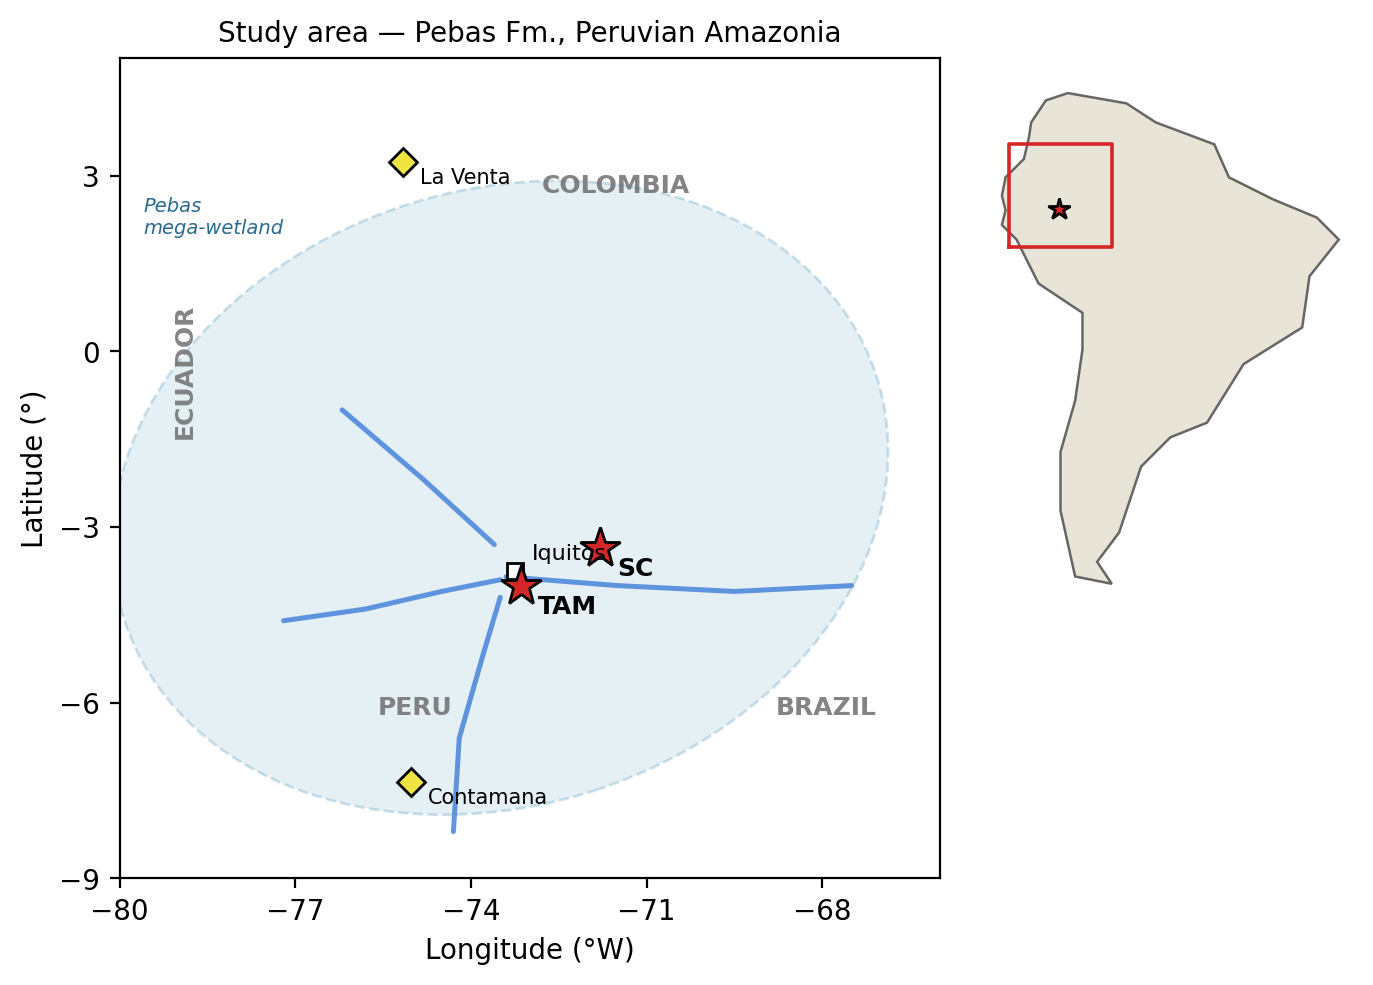
\includegraphics[width=\textwidth]{figs/fig1_location.png}\end{figure}
\begin{figure*}[t]\centering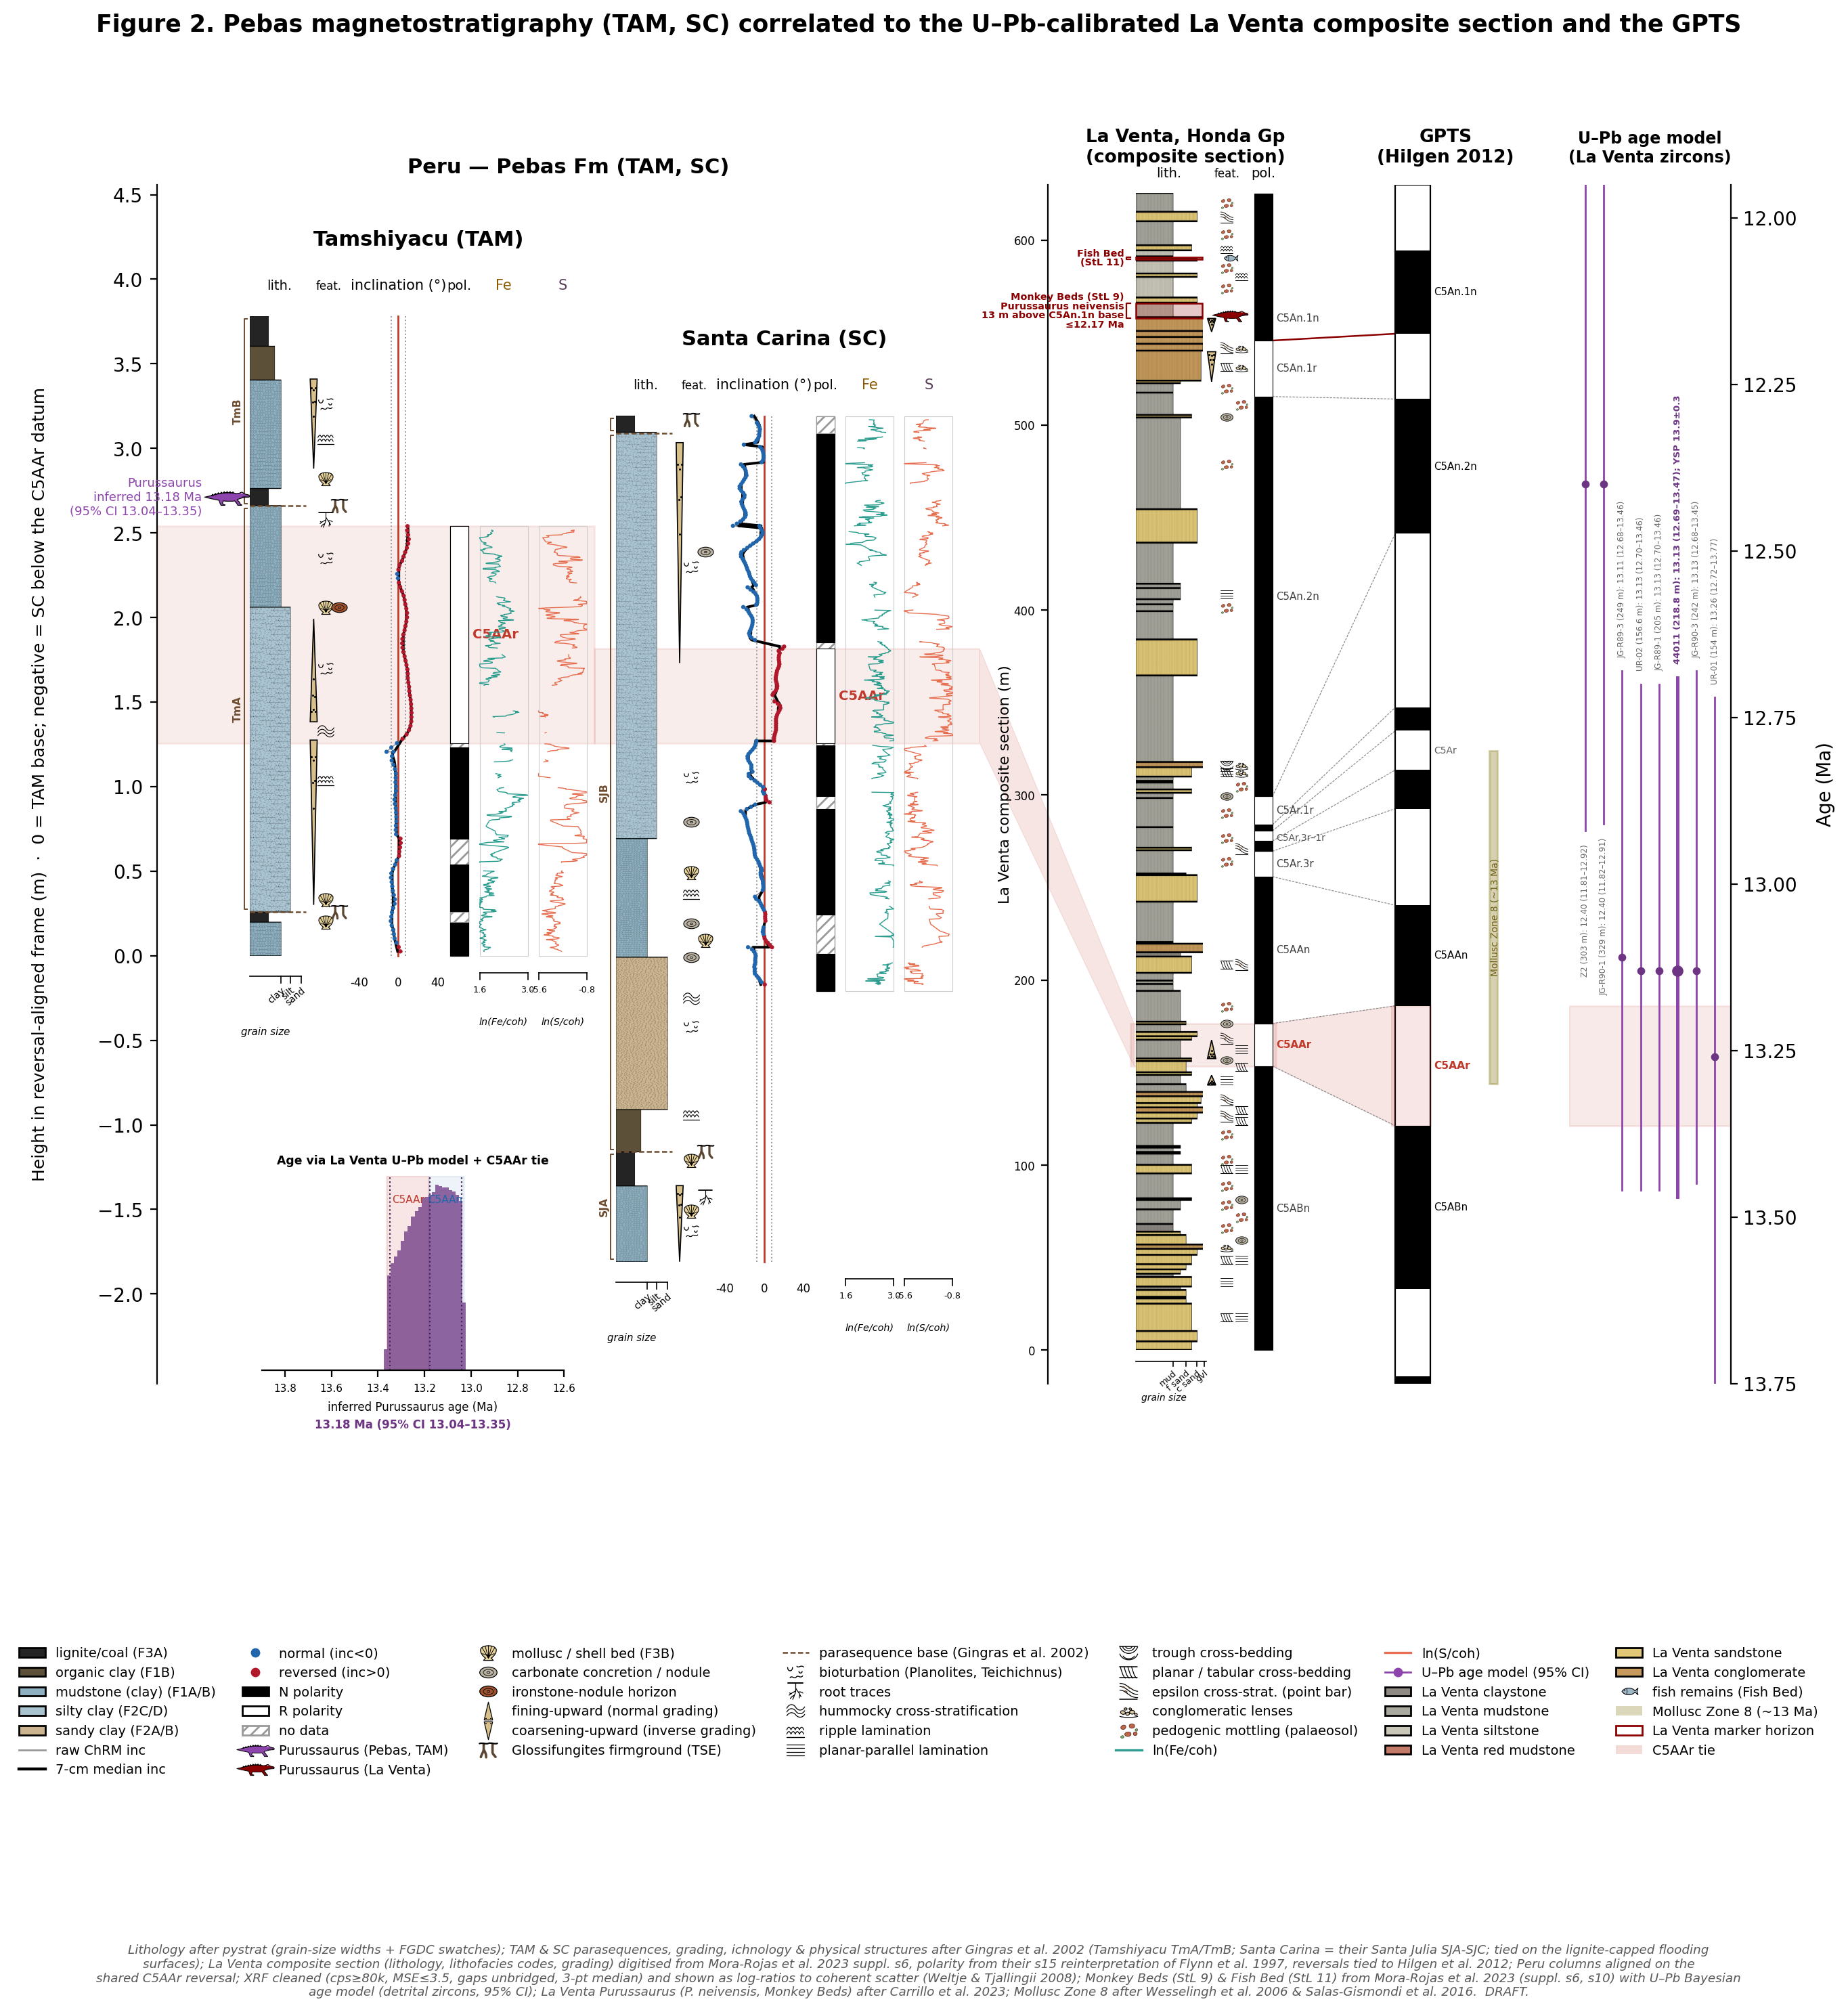
\includegraphics[width=\textwidth]{figs/fig2_master.png}\end{figure*}
\begin{figure}[t]\centering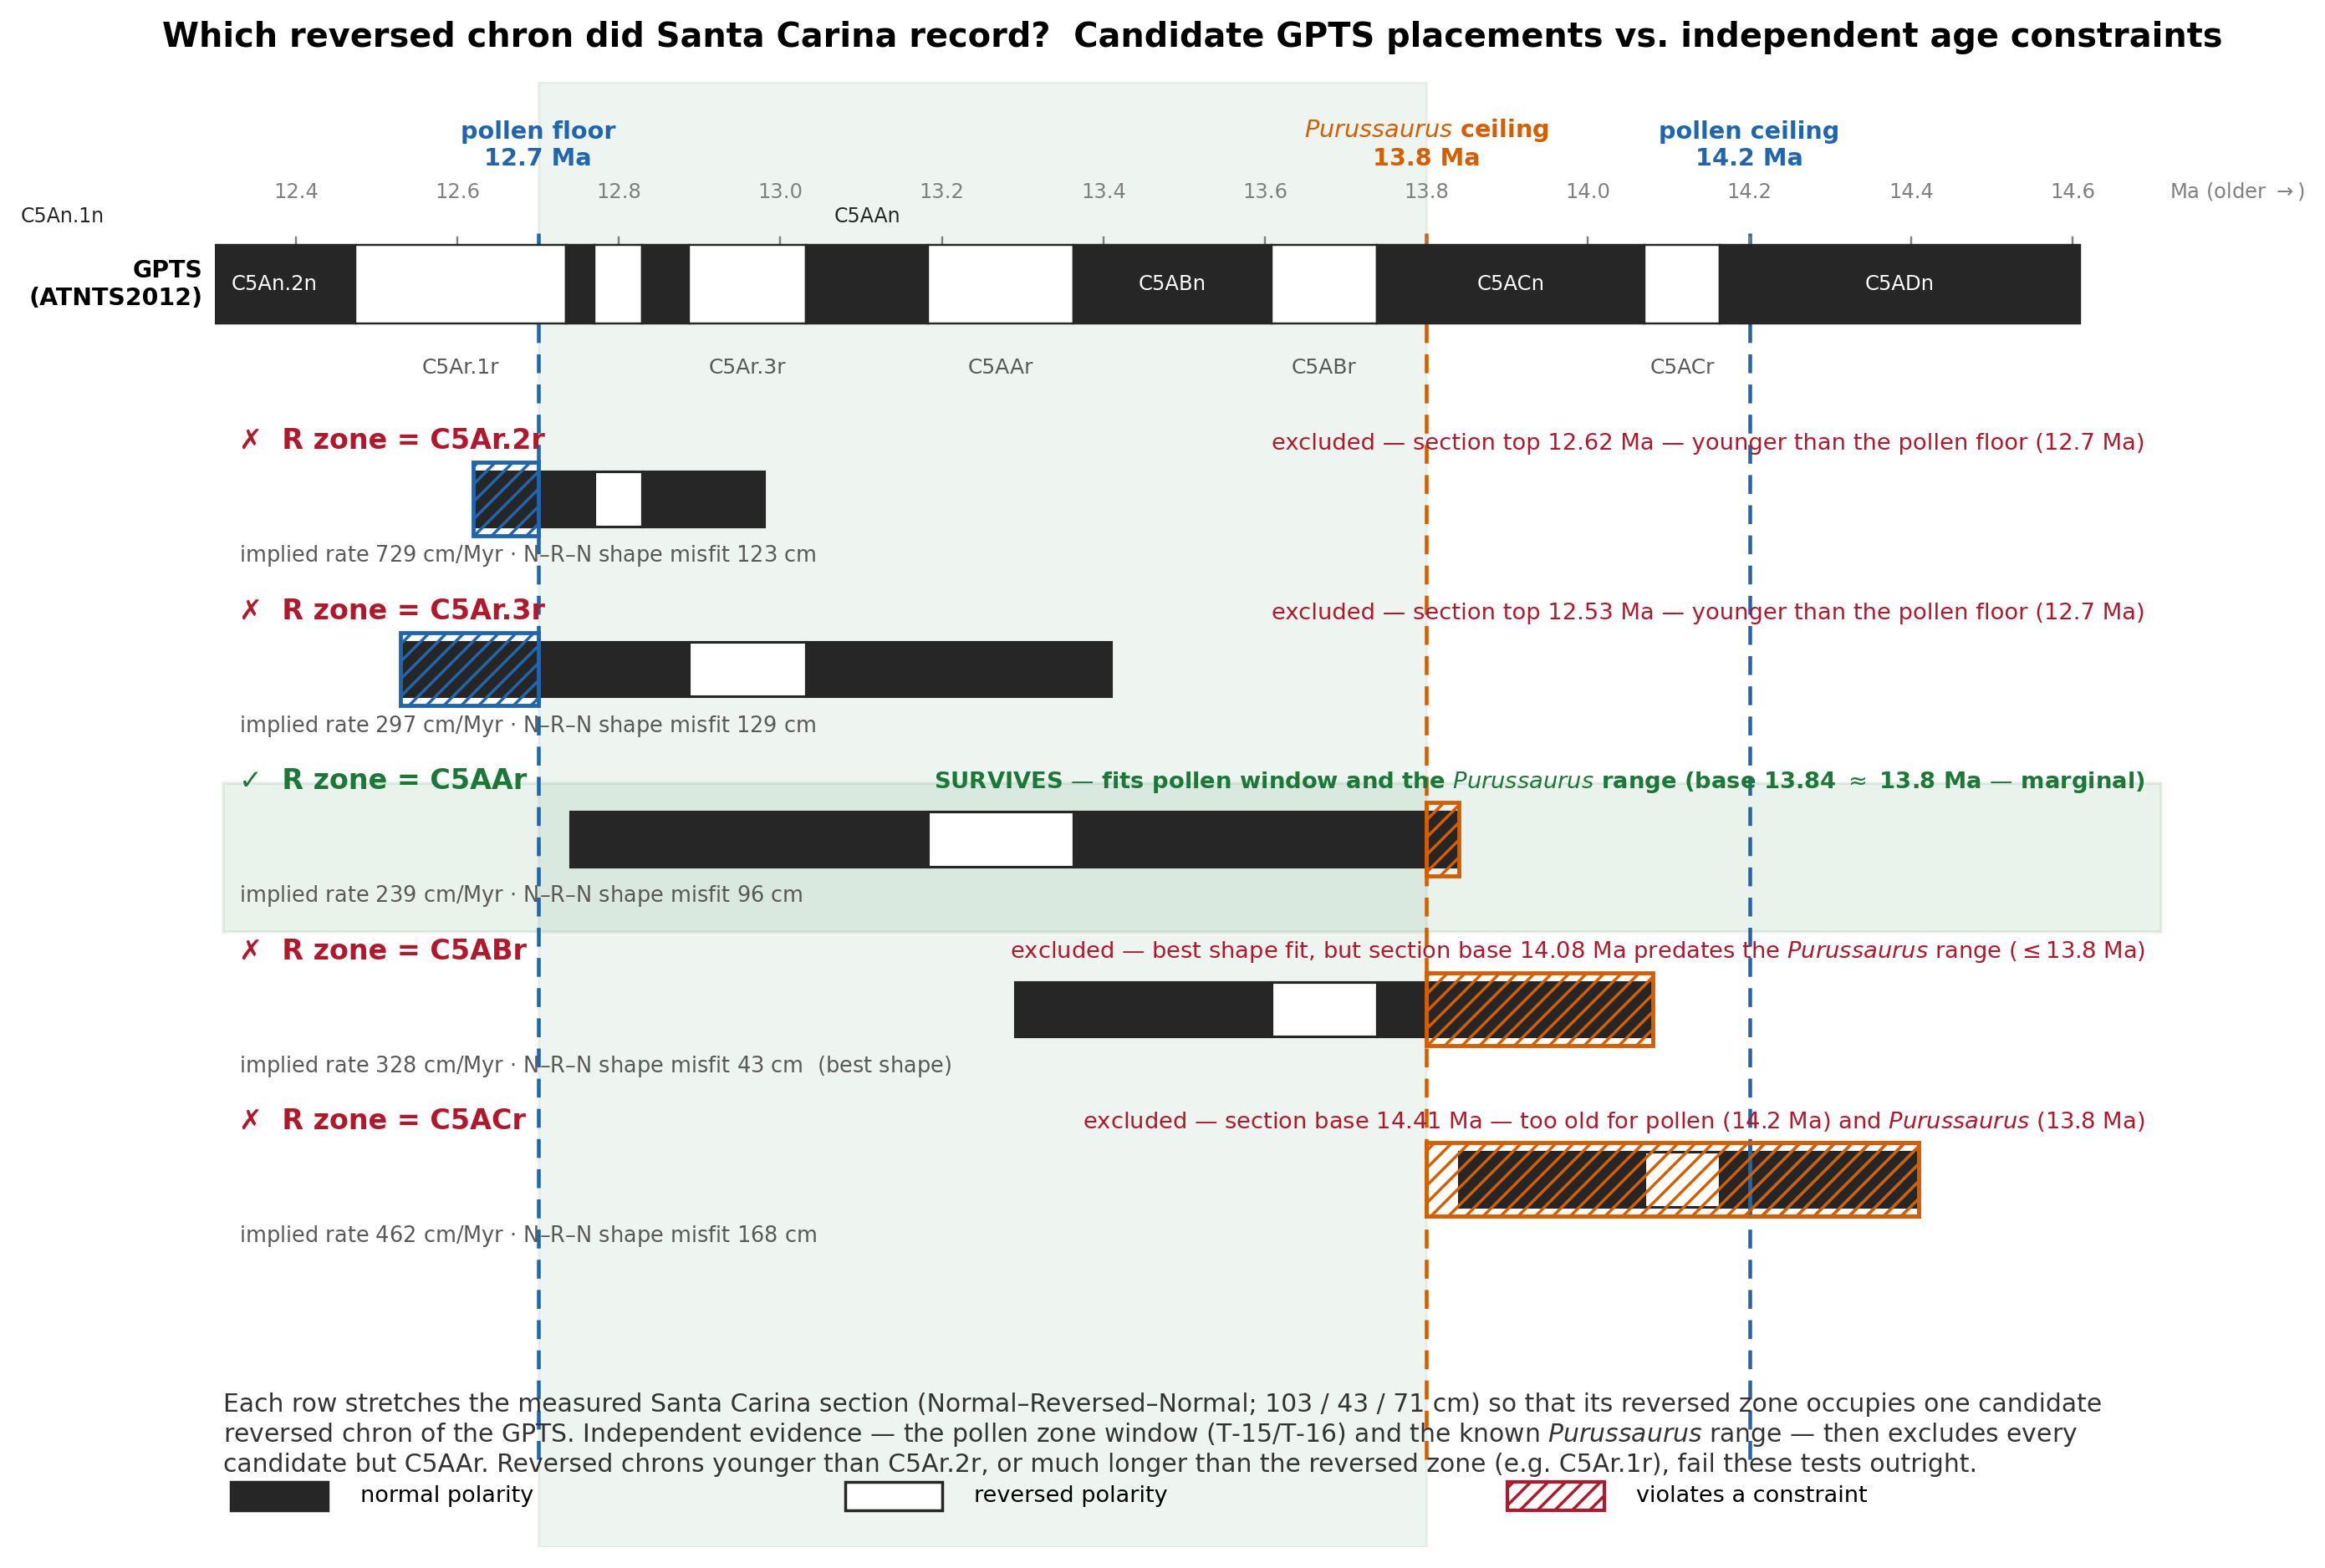
\includegraphics[width=\textwidth]{figs/fig_alternatives.png}\end{figure}
\begin{figure}[t]\centering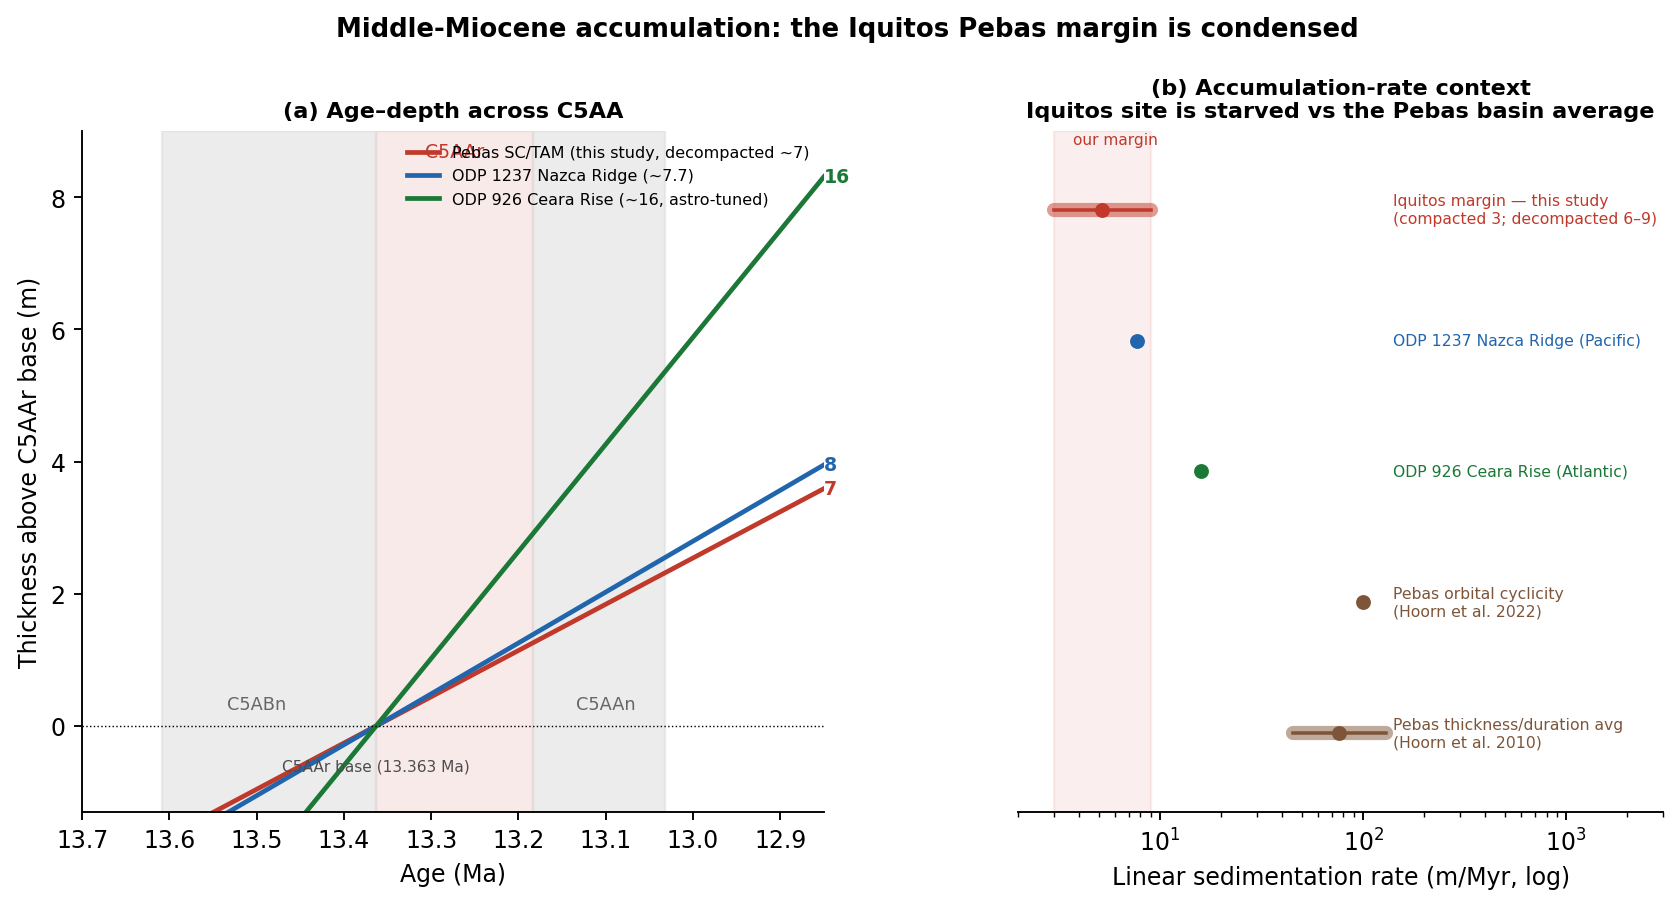
\includegraphics[width=\textwidth]{figs/fig4_sedrate.png}\end{figure}

\end{document}
